\documentclass[12pt]{article}
\usepackage{fullpage}
\usepackage{setspace}
\usepackage{amsthm}
\usepackage{amssymb}
\usepackage{tikz}
\usepackage{mathtools}
\usepackage{hyperref}
\usepackage{multicol}
\usepackage{xcolor}
\usepackage{arydshln}
\usepackage{enumitem}
\usepackage{rotating}
\usetikzlibrary{intersections}
\newcommand*\circled[1]{\tikz[baseline=(char.base)]{
            \node[shape=circle,draw,inner sep=2pt] (char) {#1};}}
\title{Math 208\\Test 1 - Solutions\\}
\date{September 20, 2013}
\author{Problems in Black\\\textcolor{red}{Answers in Red}}
\begin{document}
\maketitle
\begin{enumerate}
% Problem 1
	\item (15 Points) Find the general solution of the system \\
		$\left\{\begin{array}{rrrrrrrrrrr}
	   	 	x_1 & - & 2x_2 & + & x_3 & + & x_4 & + & x_5 & = & 2\\
	   	 	x_1 & - & 2x_2 & + & 2x_3 & - & x_4 & - & 2x_5 & = & 5\\
	   		 x_1 & - & 2x_2 & - & x_3 & + & 5x_4 & + & 7x_5 & = & 4\\
		\end{array}\right.$ \\ \\
% Answer 1
	\textcolor{red}{
	$\left[\begin{array}{rrrrr:r}
		1&-2&1&1&1&2\\
		1&-2&2&-1&-2&5\\
		1&-2&-1&5&7&4
	\end{array}\right]
	\begin{array}{c}
		R_2-R_1\\
		\longrightarrow\\
		R_3-R_1\\
	\end{array} 
	\left[\begin{array}{rrrrr:r}
		1&-2&1&1&1&2\\
		0&0&1&-2&-3&3\\
		0&0&-2&4&6&2
	\end{array}\right] 
	\begin{array}{c}
		\\
		\longrightarrow\\
		R_3+2R_2\\
	\end{array}\\
	\left[\begin{array}{rrrrr:r}
		1&-2&\hphantom{-}1&1&1&2\\
		0&0&1&-2&-3&3\\
		0&0&0&0&0&8
	\end{array}\right] 
	\begin{array}{c}
		\\
		\\
		\longleftarrow contradiction \\ 
	\end{array}$\\  \\ 
	\begin{tabular}{|r|}
		\hline
		$\therefore$ There is NO solution of the system.\\
		\hline
	\end{tabular} }
% Problem 2
	\item Let $\vec{a} =
	 	\left[ \begin{array}{r}
			3\\
			-1\\
			4\\
		\end{array}\right]$
		and $\vec{b} = 
		\left[\begin{array}{r}
			5\\
			-2\\
			1\\
		\end{array}\right]$. Find a parametric equation for the line\\
	\begin{enumerate}
	% Part (a)
		\item (5 Points) passing through (end-point of) $\vec{a}$ and parallel to $\vec{b}$;\\
	% Answer (a) 
	\textcolor{red}{
		$\vec{x}(t) = \vec{a} + t\vec{b} = 
		\left[\begin{array}{r}
			3\\
			-1\\
			4\\
		\end{array}\right] + t
		\left[\begin{array}{r}
			5\\
			-2\\
			1\\
		\end{array}\right] =  $
	\begin{tabular}{|l|}
	\hline \\
		$\left[\begin{array}{c}
			3+5t\\
			-1-2t\\
			4+t\\
		\end{array}\right]$\\ \\	
	\hline
	\end{tabular} }
	% Part (b)
		\item (5 Points) passing through the (end-points of) vectors $\vec{a}$ and $\vec{b}$\\
	% Answer (b)
		\textcolor{red}{
		$\vec{x}(t) = \vec{a} + t(\vec{b}-\vec{a}) = 
		\left[\begin{array}{r}
			3\\
			-1\\
			4\\
		\end{array}\right] + t
		\left[\begin{array}{c}
			5-3\\
			-2-(-1)\\
			1-4\\
		\end{array}\right] =  $
	\begin{tabular}{|l|}
	\hline \\
		$\left[\begin{array}{c}
			3+2t\\
			-1-t\\
			4-3t\\
		\end{array}\right]$\\ \\	
	\hline
	\end{tabular} }
	\end{enumerate}
%  Problem 3
	\item Let $\left\{\begin{array}{rrrrrrrrr}
			7x_1&+&2x_2&+&3x_3&+&5x_4&=&4\\
			x_1&-&x_2&-&2x_3&+&x_4&=&7\\
			3x_1&+&x_2&&  &-&x_4&=&-3\\
		\end{array}\right.$
	\textbf{}{Do not solve the system!}\\
	\begin{enumerate}
	% Part (a)
		\item (5 Points) Vector form \\
	% Answer (a) 
	\textcolor{red}{
	$x_1  
		\left[\begin{array}{r}
			7\\
			1\\
			3\\
		\end{array}\right]
	+ x_2  
		\left[\begin{array}{r}
			2\\
			-1\\
			1\\
		\end{array}\right]
	+ x_3  
		\left[\begin{array}{r}
			3\\
			-2\\
			0\\
		\end{array}\right]
	+ x_4  
		\left[\begin{array}{r}
			5\\
			1\\
			-1\\
		\end{array}\right]
	=
		\left[\begin{array}{r}
			4\\
			7\\
			-3\\
		\end{array}\right]$ }
	% Part (b)
		\item (5 Points) Matrix form\\
	% Answer (b)
		\textcolor{red}{
		$\left[\begin{array}{rrrr}
			7&2&3&5\\	
			1&-1&-2&1\\
			3&1&0&-1\\
		\end{array}\right]
		\left[\begin{array}{r}
			x_1\\
			x_2\\
			x_3\\
			x_4\\
		\end{array}\right] =
		\left[\begin{array}{r}
			4\\
			7\\
			-3\\
		\end{array}\right]$ }
	% Part (c)
		\item (5 Points) Augmented matrix form\\
	% Answer (c)
		\textcolor{red}{
		$\left[\begin{array}{rrrr:r}
			7&2&3&5&4\\	
			1&-1&-2&1&7\\
			3&1&0&-1&-3\\
		\end{array}\right] $ }
	\end{enumerate}
% Problem 4 
	\item (15 Points) Consider the following linear system: 
		$\left\{\begin{array}{rrrrr}
			x_1&-&hx_2&=&3\\
			2x_1&+&4x_2&=&k\\
		\end{array}\right.$
	\begin{enumerate}
	
	% Part (a)
		\item (5 Points) \hspace{1.5mm}Describe \textbf{all values} of $h$ and $k$ for which this system has exactly one solution.
	% Part (b)
		\item (5 Points) Describe \textbf{all values} of $h$ and $k$ for which this system has infinitely many solutions.
	% Part (c)
		\item (5 Points) \hspace{1.5mm}Describe \textbf{all values} of $h$ and $k$ for which this system is inconsistent.
	\end{enumerate}
% Answer 4
	\textcolor{red}{
	$\left[\begin{array}{rr:r}
		1&-h&3\\
		2&4&k\\
	\end{array}\right]
	\begin{array}{c}
		\longrightarrow\\
		R_2-2R_1\\
	\end{array}
	\left[\begin{array}{rc:c}
		1&-h&3\\
		0&4+2h&k-6\\
	\end{array}\right]$ }

	\begin{enumerate}[label=\textcolor{red}{(\alph*)}]
		\item \textcolor{red}{
			$4+2h \neq 0 \hspace{30.75mm}\leadsto\quad$ \begin{tabular}{|c|}
				\hline
				$h\neq-2,\hspace{7.5mm}k $ any\\
				\hline\end{tabular}}

		\item \textcolor{red}{$4+2h = 0 $ and $k-6 = 0 \quad\leadsto\quad$ \begin{tabular}{|c|}
				\hline
				$h=-2$ and $k=6$\\
				\hline\end{tabular} }

		\item \textcolor{red}{
			$4+2h = 0$ and $k-6 \neq 0 \quad\leadsto\quad$ \begin{tabular}{|c|}
				\hline
				$h=-2$ and $k\neq6$\\
				\hline\end{tabular} }
	\end{enumerate} 
\newpage
% Problem 5
	\item (15 Points) Find the standard matrix of the transformation $T$, where $T : \mathbb{R}^2 \longrightarrow
	\mathbb{R}^2$ first rotates by the angle $\frac{\pi}{4}$ radians (counterclockwise) 
	and then reflects with respect to the line $x_1 + x_2 = 0$.\\ 
% Answer 5

	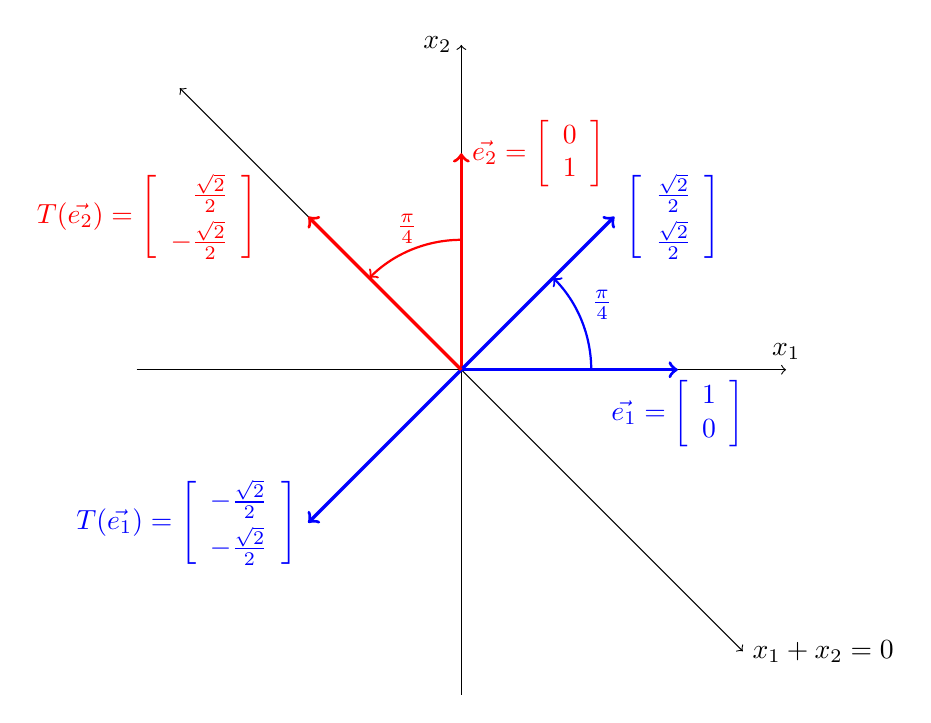
\begin{tikzpicture}[scale=2.75]
% grid
	%\draw [step=.5,gray,very thin] (-1.4,-1.4) grid (1.4,1.4);
% x-y axis
	\draw[->] (-1.5,0) -- (1.5,0) node[above]{$x_1$};
	\draw[->] (0,-1.5) -- (0,1.5) node[left]{$x_2$};
% x_1 + x_2 = 0 
	\draw[<->] (1.3,-1.3) node[right]{$x_1+x_2=0$} -- (-1.3,1.3);
% Horizontal Line 
	\draw[->,very thick,blue] (0,0) -- (1,0) node[below]
			{$\vec{e_1}=\left[\begin{array}{r}
				1\\
				0\\
			\end{array}\right]$};
% Vertical Line
	\draw[->,very thick,red] (0,0) -- (0,1) node[right]{$\vec{e_2}=\left[\begin{array}{r}
				0\\
				1\\
			\end{array}\right]$};
% Arc 1
	\draw[->,thick,blue] (6mm,0) arc (0:45:6mm);
% Arc label 1
	\node[blue] (label) at (.65,.3) {$\frac{\pi}{4}$};
% Arc 2
	\draw[->,thick,red] (0,6mm) arc (90:135:6mm);
% Arc label 2
	\node[red] (label) at (-.25,.65) {$\frac{\pi}{4}$};

% Sloped line 1
	\draw[->,very thick,blue] (0,0) -- (.707,.707) node[right]
			{$\left[\begin{array}{r}
				\frac{\sqrt{2}}{2}\vspace{1mm}\\
				\frac{\sqrt{2}}{2}\\
			\end{array}\right]$};
% Sloped line mirror
	\draw[->,very thick,blue] (0,0) -- (-.707,-.707) node[left]
			{$ T(\vec{e_1}) = 
			\left[\begin{array}{r}
				-\frac{\sqrt{2}}{2}\vspace{1mm}\\
				-\frac{\sqrt{2}}{2}\\
			\end{array}\right]$};
% Sloped line 2
	\draw[->, very thick,red] (0,0) -- (-.707,.707) node[left=.5cm]
			{$ T(\vec{e_2}) = 
			\left[\begin{array}{r}
				\frac{\sqrt{2}}{2}\vspace{1mm}\\
				-\frac{\sqrt{2}}{2}\\
			\end{array}\right]$};
\end{tikzpicture}\\
	\textcolor{red}{
	$\cos(\frac{\pi}{4}) = \frac{\sqrt{2}}{2}$, $\sin(\frac{\pi}{4}) = \frac{\sqrt{2}}{2}\\\\
		A= \left[\begin{array}{cc}
			T(\vec{e_1})&T(\vec{e_2})\\
			\vspace{5mm}\begin{rotate}{270}$\leadsto$\end{rotate}&\begin{rotate}{270}$\leadsto$\end{rotate}\\
			\end{array}\right] 
		= \left[\begin{array}{cc}
			-\frac{\sqrt{2}}{2}&-\frac{\sqrt{2}}{2}\\
			-\frac{\sqrt{2}}{2}&\frac{\sqrt{2}}{2}\\
			\end{array}\right]$ }
% Problem 6
	\item (15 Points) Find \textbf{all} values $\vec{a}$ and $\vec{b}$ for which the vectors 
		$\left[ \begin{array}{r}
			1\\
			0\\
			1\\
		\end{array}\right],
		\left[ \begin{array}{r}
			0\\
			1\\
			a\\
		\end{array}\right],
		\left[ \begin{array}{r}
			b\\
			1\\
			1\\
		\end{array}\right]$ are linearly dependent \\
% Answer 6
	\textcolor{red}{
	$\left[\begin{array}{rrr:r}
		1&0&b&0\\
		0&1&1&0\\
		1&a&1&0\\
	\end{array}\right]
	\begin{array}{c}
		\\
		\longrightarrow\\
		R_3-R_1\\
	\end{array} 
	\left[\begin{array}{rrr:r}
		1&0&b&0\\
		0&1&1&0\\
		1&a&1&0\\
	\end{array}\right] 
	\begin{array}{c}
		\\
		\longrightarrow\\
		R_3-aR_2\\
	\end{array}
	\left[\begin{array}{rrc:r}
		1&0&b&0\\
		0&1&1&0\\
		0&0&1-b-a&0\\
	\end{array}\right]$ \\ \\
	\begin{tabular}{|l|}
		\hline
		The vectors are linearly dependent if: \\
		1-b-a=0 or b=1-a\\
		\hline
	\end{tabular} }
% Problem 7
	\item (15 Points)
	 Let $T : \mathbb{R}^2 \longrightarrow \mathbb{R}^3$ be a linear transformation that maps  
		$\vec{u_1} = \left[\begin{array}{r}
		1\\
		-1\\
		\end{array}\right]$
	is
		$\vec{v_1} = \left[\begin{array}{r}
		1\\
		-2\\
		1\\
		\end{array}\right]$
	and maps
		$\vec{u_2} = \left[\begin{array}{r}
		2\\
		3\\
		\end{array}\right]$
	is
		$\vec{v_2} = \left[\begin{array}{r}
		-1\\
		1\\
		2\\
		\end{array}\right]$
	.Find the image of 
		$\vec{w} = \left[\begin{array}{r}
		1\\
		4\\
		\end{array}\right]$.\\
%Answer 7
	\textcolor{red}{
		We note that $\vec{w}=\vec{u_2}-\vec{u_1}=
			\left[\begin{array}{c}
				2\\
				3\end{array}\right]
			-\left[\begin{array}{r}
				1\\
				-1\end{array}\right]
			=\left[\begin{array}{c}
				1\\
				4\end{array}\right]$.\\
		$T(\vec{w})=T(\vec{u_2}-\vec{u_1})=T(\vec{u_2})-T(\vec{u_1})=
			\left[\begin{array}{r}
				-1\\
				1\\
				2\end{array}\right]
			-\left[\begin{array}{r}
				1\\
				-2\\
				1\end{array}\right]
			=\left[\begin{array}{r}
				-2\\
				3\\
				1\end{array}\right]\\
		\-\hspace{34.5mm}\uparrow$ Linearity\vspace{-5mm}
		\begin{center}\begin{tabular}{|c|}
			\hline\\
			$T(\vec{w})=
				\left[\begin{array}{r}
					-2\\
					3\\
					1\end{array}\right]$\\\-\\
			\hline\end{tabular}\end{center}}
%Problem 8
	\item Let $T : \mathbb{R}^2 \longrightarrow \mathbb{R}^3$. Check which of the following transformations are linear and 			which are not. \textbf{The answer should be precisely justified!}
	\begin{enumerate}
	% Part (a)
		\item (5 Points)
			$T\left(\left[\begin{array}{r}
				x_1\\
				x_2\\
			\end{array}\right]\right) =
			\left[\begin{array}{rrc}
				x_1&+&3x_2\\
				x_2&+&1\\
				\hphantom{|}x_1\\
			\end{array}\right]$\\
	% Answer (a)
		\textcolor{red}{$T\left(\left[\begin{array}{r}
				0\\
				0
			\end{array}\right]\right)=
			\left[\begin{array}{r}
				0\\
				1\\
				0
			\end{array}\right]\neq
			\left[\begin{array}{r}
				0\\
				0\\
				0
			\end{array}\right]\rightarrow$ $T$ is NOT linear}
	% Part (b)
		\item (5 Points)
			$T\left(\left[\begin{array}{r}
				x_1\\
				x_2\\
			\end{array}\right]\right) =
			\left[\begin{array}{rrr}
				x_1&+&x_2\hphantom{3}\\
				x_2&-&x_1\hphantom{3}\\
				\hphantom{|}x_1^2 &-&x_2\hphantom{3}\\
			\end{array}\right]$\\
	% Answer (b)
		\textcolor{red}{Take $\vec{u}=\left[\begin{array}{c}1\\0\\\end{array}\right], c=2\\ \begin{array}{l}
				T(2\cdot\vec{u})=T\left(2\left[\begin{array}{r}
					1\\
					0\\
				\end{array}\right]\right)=
				T\left(\left[\begin{array}{r}
					2\\
					0\\
				\end{array}\right]\right)=
				\left[\begin{array}{r}
					2\\
					-2\\
					4\\
				\end{array}\right]\hspace{-1.5mm}\begin{rotate}{315}$\leadsto$\end{rotate}\\
			2T(\vec{u})\hspace{2.5mm}=2T\left(\left[\begin{array}{r}
				1\\
				0\\
			\end{array}\right]\right)=
			2\left[\begin{array}{r}
				1\\
				-1\\
				1\\
			\end{array}\right]\hspace{3.95mm}=
			\left[\begin{array}{r}
				2\\
				-2\\
				2\\
			\end{array}\right]\begin{rotate}{45}$\leadsto$\end{rotate}\hspace{5mm}
			\end{array}T(c\vec{u})\neq cT(\vec{u})$}
	% Part (c)
		\item (5 Points)
			$T\left(\left[\begin{array}{r}
				x_1\\
				x_2\\
			\end{array}\right]\right) =
			\left[\begin{array}{rrc}
				x_1&+&2x_2\\
				x_2&-&x_1\\
				|x_1&+&x_2|\\
			\end{array}\right]$\\
	% Answer (c)
		\textcolor{red}{Take $\vec{u}=\left[\begin{array}{c}1\\0\\\end{array}\right], c=-1\\ \begin{array}{l}
				T(c\vec{u})=T\left(-\left[\begin{array}{r}
					1\\
					0\\
				\end{array}\right]\right)=
				T\left(\left[\begin{array}{r}
					-1\\
					0\\
				\end{array}\right]\right)=
				\left[\begin{array}{r}
					-1\\
					1\\
					1\\
				\end{array}\right]\hspace{-1.5mm}\begin{rotate}{315}$\leadsto$\end{rotate}\\
			cT(\vec{u})=-T\left(\left[\begin{array}{r}
				1\\
				0\\
			\end{array}\right]\right)=
			-\left[\begin{array}{r}
				1\\
				-1\\
				1\\
			\end{array}\right]\hspace{5.5mm}=
			\left[\begin{array}{r}
				-1\\
				1\\
				-1\\
			\end{array}\right]\begin{rotate}{45}$\leadsto$\end{rotate}\hspace{5mm}
			\end{array}T(c\vec{u})\neq cT(\vec{u})$}
	\end{enumerate}
% Problem 9
	\item Let $T(\vec{x}) = A\vec{x}$, where $A = 
		\left[\begin{array}{rrrrr}
			1&0&-1&0&1\\
			2&1&3&4&5\\
			0&1&5&4&3\\
		\end{array}\right]$\\
		Answer the following questions. \textbf{Justify precisely your answer. NO credit just for a guess!}
	\begin{enumerate}
	% Part (a)
		\item (5 Points) If $T : \mathbb{R}^n \longrightarrow \mathbb{R}^m$, then what is $n$ and what is $m$?\\
			\textcolor{red}{$n=5$ = number of columns\\$m=3$ = number of rows\vspace{-3mm}}
	% Part (b)
		\item (10 Points) Check if the vector
			$\left[\begin{array}{r}
				2\\
				0\\
				-1\\
			\end{array}\right] $ is in the range of $T$\\
			\textcolor{red}{$T(\vec{c})=\vec{b},\quad A\vec{x}=\vec{b}, \quad \vec{b}=
			\left[\begin{array}{r}
				2\\
				0\\
				-1\\
			\end{array}\right]\\
			\left[\begin{array}{rrrrr:r}
			1&0&-1&0&1&2\\
			2&1&3&4&5&0\\
			0&1&5&4&3&-1\\
		\end{array}\right]
		\begin{array}{c}
			R_2-2R_1\\
			\longrightarrow\\
			\\
		\end{array}
		\left[\begin{array}{rrrrr:r}
			1&0&-1&0&1&2\\
			0&1&5&4&3&-4\\
			0&1&5&4&3&3\\
		\end{array}\right]\\
		\begin{array}{c}
			\\
			\longrightarrow\\
			R_3-R_2\\
		\end{array}
		\left[\begin{array}{rrrrr:r}
			1&0&-1&0&1&2\\
			0&1&5&4&3&-4\\
			0&0&0&0&0&3\\
		\end{array}\right]
		\begin{array}{c}
			\\
			\\
			\leftarrow \textup{contradiction. $\vec{b}$ is NOT in the range of $T$.}\\
		\end{array}\\ $}
	% Part (c)
		\item (5 Points) Find the pivot entries and pivot columns of the matrix $A$\\
			\textcolor{red}{
			$\left[\begin{array}{ccrrr}
				\circled{1}&0&\hspace{-2mm}-1&0&1\\
				2&\circled{1}&3&4&5\\
				0&1&5&4&3\\
			\end{array}\right]\\
			\-\hspace{5mm}\uparrow\hspace{7mm}\uparrow$\\Pivot Columns}
	% Part (d)
		\item (5 Points) Check if $T$ is one-to-one\\
			\textcolor{red}{Number of columns of $A=5 > 2$ = number of pivot positions\\$T$ is NOT one-to-one.}
	% Part (e)
		\item (5 Points) Check if $T$ is onto\\
			\textcolor{red}{Number of rows of $A=3 > 2$ = number of pivot positions\\$T$ is NOT onto.}
	% Part (f)
		\item (5 Points) Check if the column vectors of $A$ are linearly independent.\\
			\textcolor{red}{Number of columns of $A=5 > 3$ = number of rows.\\
				Column vectors of $A$ are \underline{linearly dependent}.}
	\end{enumerate}
% *-o
\end{enumerate}

\end{document}